\section{Test-time compute before and after RL}
\label{sec:ttc}

If RL mostly concentrates probability on proofs the base can already write, then spending more compute at test time on
the base should recover part of RL's gain, and spending it on the RL model should add little. We measured two forms of
test-time compute on the full-exposure seeds s0--s2. Neither comparison below is part of the knockout. Both are
reviewed results of earlier runs (Fig.~\ref{fig:ttc}).

\begin{figure}[t]
\centering
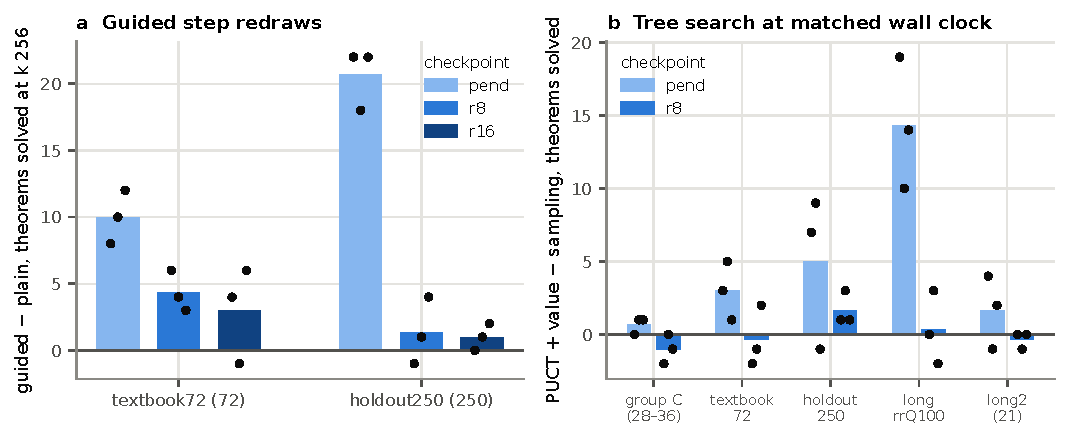
\includegraphics[width=\linewidth]{figures/fig7_ttc.pdf}
\caption{\textbf{Test-time compute helps the base, not the RL model.} (a) Guided minus plain reads, $k=256$ each, on
textbook72 and holdout250, for the base (pend) and after 8 and 16 rounds; bars are means, dots are seeds. Guided
attempts cost about 2.2 times the GPU time of plain ones, so this is not compute-matched. On holdout250 the RL models
sit within 3--14 theorems of the ceiling. (b) PUCT tree search with a learned value head minus sampling, at matched
wall-clock on the same GPU; group C holds the theorems neither pend nor r8 solves in an earlier read (28--36 per seed).}
\label{fig:ttc}
\end{figure}

\paragraph{Guided step redraws.} A guided read redraws a step that the logical checker rejects instead of abandoning
the attempt (\S\ref{sec:setup}). At $k=256$ it adds 18--22 holdout250 theorems to the base and $-1$ to $+4$ to the r8
and r16 models. The RL models are near the ceiling there, so textbook72 is the fairer pool. There guided reading adds
$+8/+10/+12$ to the base, $+6/+4/+3$ at r8 and $+4/-1/+6$ at r16. On holdout250 it halves the gap between the base and
r8, from 44/31/37 theorems (plain) to 21/14/19 (guided). The guided base solves 50--60\% of the theorems RL ``creates''
at equal $k$. These reads are not compute-matched: a guided attempt costs about 1.8 times the tokens and 2.2 times the
GPU time of a plain one. At matched sampled tokens, guided redraws still beat plain resampling on long textbook problems
on all six r8 models tested (+5.2 to +10.3 points). The six are three seeds of this recipe and three of the same
recipe trained on proofs of at most 6 lines. Guided reading does not reach most of the compute-matched creations,
however. Of the theorems RL r8 solves that the base cannot reach at $\Kpub$ (22/21/14), the guided base solves only
3/4/1.

\paragraph{Tree search.} A PUCT search over proof states, with a value head trained on the frozen policy's rollouts,
was compared with plain sampling at equal wall-clock on the same A40. At r8 it is within $\pm3$ theorems of sampling on
every pool. On group C, the theorems neither pend nor r8 solved in an earlier read, it solved 2/2/3 against sampling's
4/2/4. Its pre-registered gate ($\geq +3$ on two of three seeds) failed. A tenfold-longer exploratory read was also
level (9/5/7 vs 10/7/5). At pend, search helps on a pool of 100 long theorems (13--16 lines): $+19/+10/+14$ over
sampling. That is about 44\% of what eight EI rounds add on this pool by sampling ($+32.3$). Of the $+14.3$ mean,
$+5.3$ comes from the value head and the rest from search with the policy prior alone.

\paragraph{Reading.} Both methods recover part of RL's gain at the base and add little after RL. That is what one
expects if RL mostly converts reachable-but-unlikely proofs into likely ones. It also matches the likelihood view of
\S\ref{sec:measure}, where RL raised the hardest step of its eventual proofs from about $-6$ to about $-1$ nats.
Neither method reaches the theorems that a compute-matched base budget cannot reach. For those, step-level checking
and search over the base's own proposals do not help, consistent with the knockout's message that what the base does
not propose, RL rarely finds.
